\section{CPointer\-Predicate$<$ T $>$  Class Template Reference}
\label{classCPointerPredicate}\index{CPointerPredicate@{CPointer\-Predicate}}
{\tt \#include $<$CPointer\-Predicate.h$>$}

Inheritance diagram for CPointer\-Predicate$<$ T $>$::\begin{figure}[H]
\begin{center}
\leavevmode
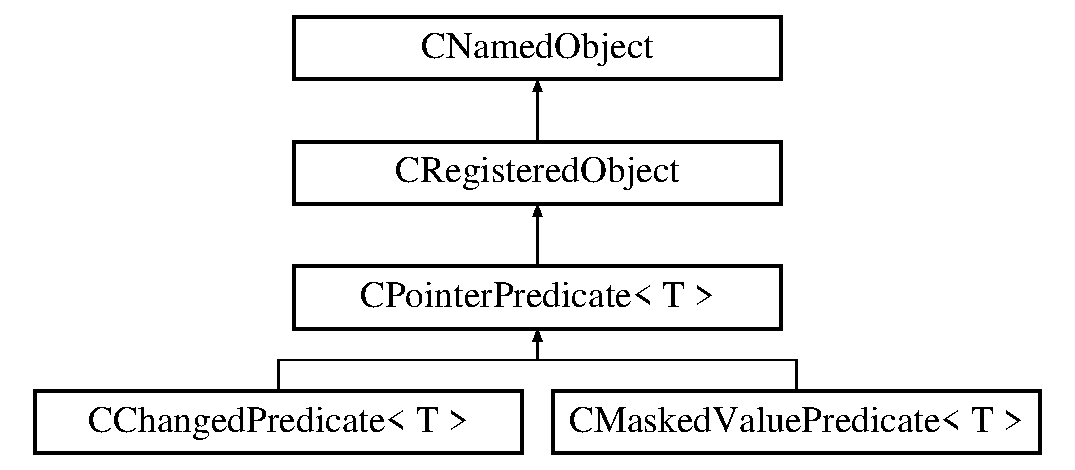
\includegraphics[height=4cm]{classCPointerPredicate}
\end{center}
\end{figure}
\subsection*{Public Methods}
\begin{CompactItemize}
\item 
{\bf CPointer\-Predicate} ()
\item 
{\bf CPointer\-Predicate} (const string \&r\-Name)
\item 
{\bf CPointer\-Predicate} (const char $\ast$p\-Name)
\item 
{\bf $\sim$CPointer\-Predicate} ()
\item 
int {\bf operator==} (const CPointer\-Predicate$<$ T $>$ \&a\-CPointer\-Predicate) const
\item 
virtual bool {\bf operator()} (T n\-Value)=0
\item 
virtual string {\bf Describe\-Self} ()=0
\end{CompactItemize}
\subsection*{Static Protected Methods}
\begin{CompactItemize}
\item 
string {\bf Get\-Auto\-Name} (const string \&r\-Base\-Name)
\end{CompactItemize}
\subsection*{Private Methods}
\begin{CompactItemize}
\item 
{\bf CPointer\-Predicate} (const CPointer\-Predicate$<$ T $>$ \&a\-CPointer\-Predicate)
\item 
CPointer\-Predicate$<$ T $>$ {\bf operator=} (const CPointer\-Predicate$<$ T $>$ \&a\-CPointer\-Predicate)
\end{CompactItemize}
\subsection*{Static Private Attributes}
\begin{CompactItemize}
\item 
unsigned int {\bf m\_\-n\-Auto\-Index} = 0
\begin{CompactList}\small\item\em Used to name autonamed objects.\item\end{CompactList}\end{CompactItemize}
\subsubsection*{template$<$typename T$>$ class CPointer\-Predicate$<$ T $>$}



\subsection{Constructor \& Destructor Documentation}
\index{CPointerPredicate@{CPointer\-Predicate}!CPointerPredicate@{CPointerPredicate}}
\index{CPointerPredicate@{CPointerPredicate}!CPointerPredicate@{CPointer\-Predicate}}
\subsubsection{\setlength{\rightskip}{0pt plus 5cm}template$<$typename T$>$ CPointer\-Predicate$<$ T $>$::CPointer\-Predicate ()\hspace{0.3cm}{\tt  [inline]}}\label{classCPointerPredicate_a0}


Used to name predicate objects \index{CPointerPredicate@{CPointer\-Predicate}!CPointerPredicate@{CPointerPredicate}}
\index{CPointerPredicate@{CPointerPredicate}!CPointerPredicate@{CPointer\-Predicate}}
\subsubsection{\setlength{\rightskip}{0pt plus 5cm}template$<$typename T$>$ CPointer\-Predicate$<$ T $>$::CPointer\-Predicate (const string \& {\em r\-Name})\hspace{0.3cm}{\tt  [inline]}}\label{classCPointerPredicate_a1}


\index{CPointerPredicate@{CPointer\-Predicate}!CPointerPredicate@{CPointerPredicate}}
\index{CPointerPredicate@{CPointerPredicate}!CPointerPredicate@{CPointer\-Predicate}}
\subsubsection{\setlength{\rightskip}{0pt plus 5cm}template$<$typename T$>$ CPointer\-Predicate$<$ T $>$::CPointer\-Predicate (const char $\ast$ {\em p\-Name})\hspace{0.3cm}{\tt  [inline]}}\label{classCPointerPredicate_a2}


\index{CPointerPredicate@{CPointer\-Predicate}!~CPointerPredicate@{$\sim$CPointerPredicate}}
\index{~CPointerPredicate@{$\sim$CPointerPredicate}!CPointerPredicate@{CPointer\-Predicate}}
\subsubsection{\setlength{\rightskip}{0pt plus 5cm}template$<$typename T$>$ CPointer\-Predicate$<$ T $>$::$\sim$CPointer\-Predicate ()\hspace{0.3cm}{\tt  [inline]}}\label{classCPointerPredicate_a3}


\index{CPointerPredicate@{CPointer\-Predicate}!CPointerPredicate@{CPointerPredicate}}
\index{CPointerPredicate@{CPointerPredicate}!CPointerPredicate@{CPointer\-Predicate}}
\subsubsection{\setlength{\rightskip}{0pt plus 5cm}template$<$typename T$>$ CPointer\-Predicate$<$ T $>$::CPointer\-Predicate (const CPointer\-Predicate$<$ T $>$ \& {\em a\-CPointer\-Predicate})\hspace{0.3cm}{\tt  [private]}}\label{classCPointerPredicate_c0}




\subsection{Member Function Documentation}
\index{CPointerPredicate@{CPointer\-Predicate}!DescribeSelf@{DescribeSelf}}
\index{DescribeSelf@{DescribeSelf}!CPointerPredicate@{CPointer\-Predicate}}
\subsubsection{\setlength{\rightskip}{0pt plus 5cm}template$<$typename T$>$ virtual string CPointer\-Predicate$<$ T $>$::Describe\-Self ()\hspace{0.3cm}{\tt  [pure virtual]}}\label{classCPointerPredicate_a6}


Describes the named object. The information given is the object type given by m\_\-s\-Class\-Path, and the object name. 

Reimplemented from {\bf CNamed\-Object} {\rm (p.\,\pageref{classCNamedObject_a8})}.

Implemented in {\bf CChanged\-Predicate$<$ T $>$} {\rm (p.\,\pageref{classCChangedPredicate_a7})}, and {\bf CMasked\-Value\-Predicate$<$ T $>$} {\rm (p.\,\pageref{classCMaskedValuePredicate_a8})}.\index{CPointerPredicate@{CPointer\-Predicate}!GetAutoName@{GetAutoName}}
\index{GetAutoName@{GetAutoName}!CPointerPredicate@{CPointer\-Predicate}}
\subsubsection{\setlength{\rightskip}{0pt plus 5cm}template$<$typename T$>$ string CPointer\-Predicate$<$ T $>$::Get\-Auto\-Name (const string \& {\em r\-Base\-Name})\hspace{0.3cm}{\tt  [static, protected]}}\label{classCPointerPredicate_e0}


$\backslash$function string {\bf CPointer\-Predicate::Get\-Auto\-Name}(const string\& r\-Base\-Name) {\rm (p.\,\pageref{classCPointerPredicate_e0})} Automatically names an object given its base class(es)\begin{Desc}
\item[Parameters: ]\par
\begin{description}
\item[{\em 
const}]string\& r\-Base\-Name The base name of the object being named \end{description}
\end{Desc}


Reimplemented from {\bf CNamed\-Object} {\rm (p.\,\pageref{classCNamedObject_e0})}.

Definition at line 296 of file CPointer\-Predicate.cpp.

References CPointer\-Predicate$<$ T $>$::m\_\-n\-Auto\-Index.\index{CPointerPredicate@{CPointer\-Predicate}!operator()@{operator()}}
\index{operator()@{operator()}!CPointerPredicate@{CPointer\-Predicate}}
\subsubsection{\setlength{\rightskip}{0pt plus 5cm}template$<$typename T$>$ virtual bool CPointer\-Predicate$<$ T $>$::operator() (T {\em n\-Value})\hspace{0.3cm}{\tt  [pure virtual]}}\label{classCPointerPredicate_a5}




Implemented in {\bf CChanged\-Predicate$<$ T $>$} {\rm (p.\,\pageref{classCChangedPredicate_a6})}, and {\bf CMasked\-Value\-Predicate$<$ T $>$} {\rm (p.\,\pageref{classCMaskedValuePredicate_a7})}.\index{CPointerPredicate@{CPointer\-Predicate}!operator=@{operator=}}
\index{operator=@{operator=}!CPointerPredicate@{CPointer\-Predicate}}
\subsubsection{\setlength{\rightskip}{0pt plus 5cm}template$<$typename T$>$ CPointer\-Predicate$<$T$>$ CPointer\-Predicate$<$ T $>$::operator= (const CPointer\-Predicate$<$ T $>$ \& {\em a\-CPointer\-Predicate})\hspace{0.3cm}{\tt  [private]}}\label{classCPointerPredicate_c1}


\index{CPointerPredicate@{CPointer\-Predicate}!operator==@{operator==}}
\index{operator==@{operator==}!CPointerPredicate@{CPointer\-Predicate}}
\subsubsection{\setlength{\rightskip}{0pt plus 5cm}template$<$typename T$>$ int CPointer\-Predicate$<$ T $>$::operator== (const CPointer\-Predicate$<$ T $>$ \& {\em a\-CPointer\-Predicate}) const\hspace{0.3cm}{\tt  [inline]}}\label{classCPointerPredicate_a4}




Definition at line 335 of file CPointer\-Predicate.h.

References CRegistered\-Object::operator==().

Referenced by CMasked\-Value\-Predicate$<$ T $>$::operator==(), and CChanged\-Predicate$<$ T $>$::operator==().

\subsection{Member Data Documentation}
\index{CPointerPredicate@{CPointer\-Predicate}!m_nAutoIndex@{m\_\-nAutoIndex}}
\index{m_nAutoIndex@{m\_\-nAutoIndex}!CPointerPredicate@{CPointer\-Predicate}}
\subsubsection{\setlength{\rightskip}{0pt plus 5cm}template$<$typename T$>$ unsigned int CPointer\-Predicate$<$ T $>$::m\_\-n\-Auto\-Index = 0\hspace{0.3cm}{\tt  [static, private]}}\label{classCPointerPredicate_r0}


Used to name autonamed objects.

Named\-Object.cpp Base class for all objects in the event management system.

Author: Jason Venema NSCL Michigan State University East Lansing, MI 48824-1321 mailto:{\tt venemaja@msu.edu} 

Reimplemented from {\bf CNamed\-Object} {\rm (p.\,\pageref{classCNamedObject_r0})}.

Definition at line 283 of file CPointer\-Predicate.cpp.

Referenced by CPointer\-Predicate$<$ T $>$::Get\-Auto\-Name().

The documentation for this class was generated from the following files:\begin{CompactItemize}
\item 
{\bf CPointer\-Predicate.h}\item 
{\bf CPointer\-Predicate.cpp}\end{CompactItemize}
